% !TEX root = ../CategoricalCoDesign.tex
\section{Thinking about how things transform into each other}

\subsection{Category theory helps reasoning about interfaces and transformations}

We argue that all the concepts of formal engineering design discussed in the
previous section can be naturally described in the language of category theory. We will start with a simple example. In an electric car, electric power is turned by the engine into rotational
motion of the axle, and then the rotational motion is converted into translational motion by the wheels and their friction with the road. In this simple setting, we can identify the key systems and subsystems: car, engine, axle, wheels, and road.

We can identify the functionality/resources of interest as: $\mathsf{electric} \ \mathsf{power}$, $\mathsf{rotational}\ \mathsf{motion}$, and $\mathsf{translational}\ \mathsf{motion}$. Note that each of these quantities plays a dual role. For example, the $\mathsf{rotational} \ \mathsf{motion}$ is something which is produced by the motor, so it is a functionality for the motor, while it is a resource for axle/wheels, because they need it to provide $\mathsf{translational}\ \mathsf{motion}$.

For a first qualitative description of the scenario, we might choose to just keep track of what functionality/resource is converted into what. For this qualitative description, we can draw a diagram in which each resource
is a point (\cref{fig:e1}).

\begin{figure}[h!]
    \centering
    \includesag{30_dpcatfig_e1}
    \caption{Resources and functionalities in the electric car example. \label{fig:e1}}
\end{figure}

Furthermore, we can draw an arrow between two resources if we can obtain one
from the other. In the example, we have described how $\mathsf{electric}\ \mathsf{power}$ becomes $\mathsf{rotational}\
\mathsf{motion}$, described by the $\mathsf{engine}$ arrow, and how $\mathsf{rotational}\
\mathsf{motion}$ becomes $\mathsf{translational}\ \mathsf{motion}$, described by the $\mathsf{wheel}$ arrow (\cref{fig:e2}).
\GZ{AC: direction of arrows should be coherent with later definition of DP, res to fun}

\begin{figure}[h!]
    \centering
    \includesag{30_dpcatfig_e2}
    \caption{System components connect resources and functionalities- \label{fig:e2}}
\end{figure}

In this representation, the arrows are the components of the system.
We will learn how to compose these arrows according to the rules of category theory.

If we use the semantics that an arrow from resource $X$ to resource $Y$ means ``having $Y$ is
enough to obtain $X$'', then, since $Y$ is enough for $Y$ per definition, we can add a self-loop for each
resource. We will call the self-loops \emph{identities} (\cref{fig:e3}).

\begin{figure}[h!]
    \centering
    \includesag{30_dpcatfig_e3}
    \caption{System components and identities. \label{fig:e3}}
\end{figure}

Furthermore, we might consider the idea of composition of arrows. If from $Y$ we
can get $X$ and from $Z$ we can get $Y$, then from $Z$ we can get $X$. In our
example, if the arrows $\mathsf{wheel}$ and $\mathsf{engine}$ exist, then also the arrow ``$\mathsf{engine}$ then $\mathsf{wheel}$''
exists~(\cref{fig:e4}).

\begin{figure}[h!]
    \centering
    \begin{tikzcd}
\bullet \arrow[bend left = 30, rr, "\wheels\text{ then }\motor"] \arrow[out=120,in=60,loop,looseness=5]\arrow[r,"\wheels"] & \bullet \arrow[r,"\motor"] \arrow[out=120,in=60,loop,looseness=5]& \bullet  \arrow[out=120,in=60,loop,looseness=5]\\[-15pt]
    \translationalmotion&\rotationalmotion&\electricpower
\end{tikzcd}
    \caption{Composition of system components \label{fig:e4}.}
\end{figure}

\GZ{Figure has to go here}


A ``category'' is an abstract mathematical
structure which captures the intuitive notions of objects and arrows between them.
The following is the formal definition.

\begin{shaded}
\begin{definition}[Category] \label{def:categorymain}
A \emph{category} $\CatC$ is specified by four components:
%vthe
%category's \emph{objects}, the category's \emph{morphisms},
%the \emph{identities} and the \emph{composition operations}. More precisely,
%a category consists of:
\begin{compactenum}
\item \emph{Objects}: a collection\footnotemark \  $\ObC$, whose elements are called \emph{objects}.
\item \emph{Morphisms}: for every pair of objects $X, Y\in \ObC$, there is a set $\CatC(X, Y)$, the elements of which are called
\emph{morphisms} from $X$ to $Y$.
\item \emph{Identity morphisms}:  for each object $X$, there is
an element $\id_X \in \HomC(X,X) $ which is called \emph{the identity
morphism of $X$}.
\item \emph{Composition operations}: given any morphism $f \in  \HomC(X,Y) $ and any morphism $g \in \HomC(Y, Z)$, there exists a morphism $f\then g$ in $\HomC(X, Z)$ which is the \emph{composition of $f$ and $g$}.
\end{compactenum}

\

Furthermore, these constituents are required to satisfy the following conditions:

\

\begin{compactenum}
    \item \emph{Unitality}: for any morphism $f\in\Hom(X,Y)$,
    \begin{equation}
        \id_X \then f= f = f \then \id_Y.
    \end{equation}
    \item \emph{Associativity}: for $f\in \HomC(X,Y)$, $g\in \HomC(Y,Z)$, and $h\in \HomC(Z,W)$,
    \begin{equation}
        (f\then g)\then h= f \then (g \then h).
    \end{equation}
\end{compactenum}

\end{definition}
\end{shaded}
\footnotetext{A ``collection'' is something which may be thought of as a set, but may be ``too large" to technically be a set in the formal sense. This distinction is necessary in order to avoid such issues as Russel's paradox.}

\begin{remark}
The set of morhisms $\CatC(X, Y)$ is sometimes denoted $\HomC(X, Y)$ and called the ``hom-set from $X$ to $Y$''. The ``Hom'' comes from the word ``homomorphism''.
\end{remark}

\begin{remark}[Composition notation]
We denote composition of morphisms in a somewhat unusual way--sometimes preferred by category-theorists and computer scientists--namely in \emph{diagrammatic order}. That is, given~$f\colon A\to B$ and~$g\colon B\to C$, we denote their composite by~$(f\then g)\colon A\to C$, pronounced ``$f$ then $g$''. This is in contrast to the more typical notation for composition, namely~$g\circ f$, or simply~$gf$, which reads as ``$g$ after $f$''. The notation~$f\then g$ is sometimes called \emph{infix notation}.
\end{remark}

Note that we may save some ink when drawing diagrams of morphisms:
\begin{compactitem}
\item We do not need to draw the identity arrows from one object to itself, because, by \cref{def:categorymain}, they always exist.
%However, we will see how there might be multiple such loops.
\item  Given arrows~$A\to B$ and~$B \to C$, we do not need to draw their composition because, by \cref{def:categorymain}, this composition is guaranteed to exist.
\end{compactitem}

With these conventions, we can just draw the arrows~$\mathsf{engine}$ and~$\mathsf{wheel}$ in the diagram, and the rest of the diagram is implied (\cref{fig:e5}).

\begin{figure}[h!]
    \centering
    \includesag{30_dpcatfig_e5}
    \caption{Electric car example. The grey arrows are implied by the properties
    of a category.\label{fig:e5} }
\end{figure}

Particularly, the electric car example corresponds to the category~$\CatC$ specified by
\begin{itemize}
    \item \emph{Objects:} $\Ob_\CatC=\{\mathsf{electric}\ \mathsf{power},\mathsf{rotational}\ \mathsf{motion},\mathsf{translational}\ \mathsf{motion}\}$.
    \item \emph{Morphisms}: The system components are the morphisms. For instance, we have $\mathsf{engine}$, $\mathsf{wheel}$, and the morphism $\mathsf{wheel \then engine}$, implied by the properties of the category.
\end{itemize}

We can slightly expand this example by noting the inverse transformations. In an electric car
it is possible to regenerate power; that is, we can obtain $\mathsf{rotational}\ \mathsf{motion}$ of the wheels from
$\mathsf{translational}\ \mathsf{motion}$ (via the morphism $\mathsf{move}$), and then convert the $\mathsf{rotational}\ \mathsf{motion}$ into $\mathsf{electric}\ \mathsf{power}$ (via the morphism $\mathsf{dynamo}$)~(\cref{fig:e6},~\cref{fig:e6-together}).

\begin{figure}[h!]
    \centering
    \includesag{30_dpcatfig_e6}
    \caption{\label{fig:e6}}
\end{figure}


\GZ{Conflict in composition order in figures, discuss on how to fix}
\begin{figure}[h!]
    \centering
    \includesag{30_dpcatfig_e7}
    \caption{\label{fig:e6-together}}
\end{figure}
\GZ{reformulate using axiom of comp in cat}
Given the semantics of the arrows in a category, all compositions of arrows exist, even if they are not drawn
explicitly. For example, we can consider the composition~$f\then g \then k \then h$, which
converts $\mathsf{electric}\ \mathsf{power}$ into $\mathsf{rotational}\ \mathsf{motion}$, into $\mathsf{translational}\ \mathsf{motion}$, then back to
$\mathsf{rotational}\ \mathsf{motion}$ and $\mathsf{electric}\ \mathsf{power}$. Note that this is an arrow that has the same head and tail as the identity arrow on $\mathsf{electric}\ \mathsf{power}$~(\cref{fig:e8}). However, these two arrows are not necessarily the same. In this example we are representing physical systems, so we would in fact not expect them to be the same, since there will be some losses during the many conversions.

\begin{figure}[h!]
    \centering
    \includesag{30_dpcatfig_e8}
    %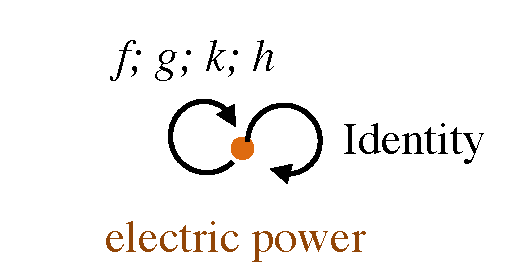
\includegraphics[scale=0.33]{dpcatfig_e8}
    \caption{\label{fig:e8}}
\end{figure}

It is important to recognize that there might also be two or more distinct arrows between two distinct resources~(\cref{fig:e9}). Each arrow between $X$ and $Y$ represents a different way  to obtain~$X$ from~$Y$. This is one of the aspects which will make category theory powerful enough to reason about design.

\begin{figure}[h!]
    \centering
    \includesag{30_dpcatfig_e9}
    \caption{\label{fig:e9}}
\end{figure}

The directionality of the arrows is also important. While the convention of
which resource is the tail and which the head is just a typographic convention,
it might be the case that we know how to convert one resource into another, but
not vice versa. \cref{fig:e10} shows an example of a diagram that describes a process which is definitely
not invertible.

\begin{figure}[h!]
    \centering
    \includesag{30_dpcatfig_e10}
    \caption{An example of a process which is not invertible. \label{fig:e10}}
\end{figure}

\subsection{Currency categories}
In this section, we introduce a kind of category for describing currency exchangers. Our idea is to model currencies as objects of a category, and morphisms will describe ways of exchanging between those currencies, \text{e.g.} as offered by a currency exchange service. 

We start with a set $\mathsf{C}$ of labels for all the currencies we wish to consider, \text{i.e.} 
\begin{equation*}
    \mathsf{C} = \{ \text{EUR}, \text{USD}, \text{CHF}, \text{SGD}, ... \}.
\end{equation*}
For each currency $\mathsf{c} \in \mathsf{C}$ we define an object $\mathbb{R} \times \{c\}$ which represents possible amounts of the given currency $\mathsf{c}$ (we will ignore the issue of rounding currencies to an accuracy of two decimals places, and we allow negative amounts). The currency label keeps track of which ``units'' we are using.

Now consider two such objects, say $\mathbb{R} \times \{\text{USD}\}$ and $\mathbb{R} \times \{\text{EUR}\}$. How can we describe the process of changing an amount of USD to an amount of EUR? We model this using two numbers: an exchange rate $a_{\text{USD}, \text{EUR}}$ and a commission $b_{\text{USD}, \text{EUR}}$ for the transaction. Given an amount $x \in \mathbb{R}$ of USD, we define a morphism (a currency exchanger)
\begin{equation*}
E_{a,b} \colon \mathbb{R} \times \{\text{USD}\} \rightarrow \mathbb{R} \times \{\text{EUR}\}
\end{equation*}
by the formula
\begin{equation*}
\tup{x, \text{USD}} \longmapsto \tup{ax - b, \text{EUR}}. 
\end{equation*}
(Note that that the commission is given in the units of the target currency.) Of course, for changing USD to EUR, there may be various different banks or agencies which each offer different exchange rates and/or different commissions. Each of these corresponds to a different morphism from $\mathbb{R} \times \{\text{USD}\}$ to $\mathbb{R} \times \{\text{EUR}\}$.

To build our category, we also need to specify how currency exchangers compose. Given currencies $\mathsf{c_1}, \mathsf{c_2}, \mathsf{c_3}$, and given currency exchangers
\begin{equation*}
E_{a,b} \colon \mathbb{R} \times \{\mathsf{c_1} \} \rightarrow \mathbb{R} \times \{ \mathsf{c_2}\}
\qquad \text{and} \qquad
E_{a',b'} \colon \mathbb{R} \times \{\mathsf{c_2}\} \rightarrow \mathbb{R} \times \{\mathsf{c_3}\}
\end{equation*}
we define the composition $E_{a,b} \then E_{a',b'}$ to be the currency exchanger
\begin{equation}\label{comp law curr}
E_{aa',a'b + b'} \colon \mathbb{R} \times \{\mathsf{c_1}\} \rightarrow \mathbb{R} \times \{\mathsf{c_3}\}.
\end{equation}
In other words, we compose currency exchangers as one would expect: we multiply the first and the second exchange rates together, and we add the commissions (paying attention to first transform the first commission into the units of the final target currency).

Finally, we also need to specify unit morphisms for our category. These are currency exchangers which ``do nothing''. For any object $\mathbb{R} \times \{ \mathsf{c}\}$, its identity morphism is 
\begin{equation*}
E_{1,0} \colon \mathbb{R} \times \{\mathsf{c}\} \rightarrow \mathbb{R} \times \{\mathsf{c}\},
\end{equation*}
the currency exchanger with exchange rate ``1''  and commission ``0''. 

It is a straightforward to check that the composition of currency exchangers as defined above obeys the associative law, and that the identity morphisms act neutrally for composition. Thus we indeed have a category!

\begin{remark}
In the above specification of our category of currency exchangers, we can actually just work with the set of currency labels $\mathsf{C}$ as our objects, instead of using ``amounts'' of the form $\mathbb{R} \times \{\mathsf{c}\}$ as our objects. Indeed, on a mathematical level, the definition of currency exchangers and their composition law (\cref{comp law curr}) do not depend on using amounts! Namely, a currency exchanger $E_{a,b}$ is specified by the pair of numbers $\tup{a, b}$, and the composition law (\ref{comp law curr}) may then, in this notation, be written as 
\begin{equation}
\begin{aligned}
\label{eq:currencycomp}
    \tup{a,b}\then \tup{a',b'}&=\tup{a' a, a' b + b'}.
\end{aligned}
\end{equation}
The interpretation is still that currency exchangers change amounts of one currency to amounts in an another currency, but for this we don't need to carry around copies of $\mathbb{R}$ in our notation.
\end{remark}

Following the above remark: 

\begin{definition}[Category of currencies]
    A \emph{category of currencies} is specified by:
    \begin{compactenum}
        \item \emph{Objects:} a collection of currencies $\mathsf{C}$.
        \item \emph{Morphisms:} given two currencies $\mathsf{c_1},\mathsf{c_2}\in \mathsf{C}$, morphisms between them are currency exchangers $\tup{a,b}$ from $\mathsf{c_1}$ to $\mathsf{c_2}$.
        \item \emph{Identity morphism:} given an object $\mathsf{c} \in \mathsf{C}$, its identity morphism is the currency exchanger $\tup{1,0}$. We also call such morphisms ``trivial currency exchangers''.
        \item \emph{Composition of morphisms:} the composition of morphisms is given by the formula (\ref{eq:currencycomp}).    \end{compactenum}
\end{definition}

As an illustration, consider three currency exchange companies $\mathsf{ExchATM}$, $\mathsf{MoneyLah}$, and $\mathsf{Frankurrencies}$, which operate on several currencies (\cref{tab:currencycompanies}).

\begin{table}[h]
    \centering
    \begin{tabular}{c|c|c|c|c}
         Company name& Exchanger label & Direction &$a$ (exchange rate)&$b$   (fixed commission)  \\
         \hline
         $\mathsf{ExchATM}$&$A$&USD to CHF&\unitfrac[0.95]{CHF}{USD}&\unit[2.0]{CHF}\\
         $\mathsf{ExchATM}$&$B$&CHF to USD&\unitfrac[1.05]{USD}{CHF}&\unit[1.5]{USD}\\
         $\mathsf{ExchATM}$&$C$&USD to SGD&\unitfrac[1.40]{SGD}{USD}&\unit[1.0]{SGD}\\
         $\mathsf{MoneyLah}$&$D$&USD to CHF&$\unitfrac[1.00]{CHF}{USD}$&\unit[1.0]{CHF}\\
         $\mathsf{MoneyLah}$&$E$&SGD to USD&\unitfrac[0.72]{USD}{SGD}&\unit[3.0]{USD}  \\
        $\mathsf{Frankurrencies}$&$F$& EUR to CHF&\unitfrac[1.20]{CHF}{EUR}&\unit[0.0]{CHF}\\
        $\mathsf{Frankurrencies}$&$G$& CHF to EUR&\unitfrac[1.00]{EUR}{CHF}&\unit[1.0]{EUR}
    \end{tabular}
    \caption{Three currency exchange companies operating different currencies.
    }
    \label{tab:currencycompanies}
\end{table}
We can represent this information as a graph, where the nodes are the currencies and the edges are particular exchange operations (\cref{fig:currencygraph}). 

\begin{figure}[h]
\begin{center}
    \begin{tikzcd}[column sep = 5cm, row sep = 3cm]
    \text{USD}\arrow[bend left=20, r,"A"]\arrow[bend right=20, r,"D",swap]
    \arrow[d,bend left=20,"C"]
    &\text{CHF}
    \arrow[d,bend left=20,"G"]
    \arrow[l,"B"]\\
    \text{SGD}\arrow[u,bend left=20,"E"]&
    \text{EUR}
    \arrow[u,bend left=20,"F"]
    \end{tikzcd}
\end{center}
\caption{Three currency exchange companies operating different currencies as a graph. \label{fig:currencygraph}}
\end{figure}

There is a currency category built from the information in \cref{tab:currencycompanies} and the graph in \cref{fig:currencygraph}. Its collection of objects is the set $\{  \text{EUR}, \text{USD}, \text{CHF}, \text{SGD} \}$, and it morphisms are, in total, 
\begin{itemize}
\item the trivial currency exchanger (identity morphism) $\tup{1,0}$ for each of the four currencies (which are the objects),
\item the currency exchangers corresponding to each item in \cref{tab:currencycompanies},
\item all possible compositions of the currency exchangers listed in \cref{tab:currencycompanies}.
\end{itemize}

The phrase ``all possible compositions'' is a bit vague. What we mean here can be made more precise. It corresponds to a general recipe for starting with a graph $G$, such as in \cref{fig:currencygraph}, and obtaining from it an associated category, called the \emph{free category on} $G$. We introduce this concept in the next section. 

%The graph representation seems enough to describe this as a category, where the objects are the currencies (USD,CHF,EUR, and SGD), the morphisms are the different exchange operations, and the identity morphisms are identity currency exchangers. However, to properly define this category, we need to define composition and prove that the category is closed with respect to it, i.e. that the composition of two currency exchangers is a currency exchanger in the category. Given three currencies $\mathsf{X,Y,Z}$, a currency exchanger $\tup{a,b}$ from $\mathsf{X}$ to $\mathsf{Y}$, and a currency exchanger $\tup{c,d}$ from $\mathsf{Y}$ to $\mathsf{Z}$, one can define their composition as
%\begin{equation}
%\begin{aligned}
%\label{eq:currencycomp}
%    \tup{a,b}\then \tup{c,d}&=\tup{c\cdot a,c\cdot b+d}
%\end{aligned}
%\end{equation}
%Note that the result of the composition of currency exchangers is a currency exchanger: Thus, currency exchangers are closed under the composition operation we have defined. Finally, we need to check \emph{unitality} and \emph{associativity} for composition. Given a currency exchanger $\tup{a,b}$ from $\mathsf{X}$ to $\mathsf{Y}$ one has
%\begin{equation}
%    \begin{aligned}
%    \tup{1,0}\then \tup{a,b}&=\tup{a,b}\then \tup{1,0}\\
%    &=\tup{a,b},
%    \end{aligned}
%\end{equation}
%which is unitality. Furthermore, given a currency exchanger $\tup{c,d}$ from $\mathsf{Y}$ to $\mathsf{Z}$ and a currency exchanger $\tup{e,f}$ from $\mathsf{Z}$ to $\mathsf{W}$, one has
%\begin{equation}
%    \begin{aligned}
%    (\tup{a,b}\then \tup{c,d})\then \tup{e,f}&=\tup{a,b}\then( \tup{c,d}\then \tup{e,f})\\
%    &=\tup{eca, ecb+ed+f},
%    \end{aligned}
%\end{equation}
%which is associativity.
%We are now ready to properly define the category of currency exchangers $\mathbf{Curr}$.
%
%\begin{definition}[Category of currencies]
%    The \emph{category of currencies} $\mathbf{Curr}$ is specified by:
%    \begin{compactenum}
%        \item \emph{Objects:} $\Ob_\mathbf{Curr}$ is a collection of currencies.
%        \item \emph{Morphisms:} Given two currencies $\mathsf{C},\mathsf{D}\in \Ob_{\mathbf{Curr}}$, morphisms between them are currency exchangers $\tup{a,b}$ from $\mathsf{C}$ to $\mathsf{D}$.
%        \item \emph{Identity morphism:} Given an object $C\in \Ob_\mathbf{Curr}$, the identity morphism is given by the currency exchanger $\tup{1,0}$.
%        \item \emph{Composition of morphisms:} The composition of morphisms is given by composition of currency exchangers.
%    \end{compactenum}
%\end{definition}


\JL{The following paragraph(s) might be best moved to a later part in the text, once pareto fronts and optimization have been discussed a little bit.}
The category $\Cat{Curr}$ represents the set of all possible currency exchangers that could
ever exist. However, in this set there would be very irrational agents. For example, there is a currency exchanger that given 1 USD, will give you back 2 USD, or even will not give you back any money. This highlights a recurring topic: often mathematicians will be happy to define a broader category of objects, while, in practice, the engineer will find herself thinking about a more constrained set of objects. In particular, one would like to find the best conversions. These can be expressed as \emph{Pareto fronts}. To do so, one only needs to iterate a finite number of times, since the optimal path (conversion morphism), if such a morphism exists, will never pass through the same currency more than once. \JL{the previous sentence needs explaining} This is valid if we assume the action of converting back and forth the same currency to have a cost (through the commission) higher than 0. To see this, consider three currencies $\mathsf{A,B,C}$, a currency exchanger $\tup{a,b}$ from $\mathsf{A}$ to $\mathsf{B}$ , a currency exchanger $\tup{c,d}$ from $\mathsf{B}$ to $\mathsf{C}$ , and a currency exchanger $\tup{e,f}$ from $\mathsf{C}$ to $\mathsf{A}$. \JL{more pedagogical} The composition of the currency exchangers reads:
\begin{equation*}
\tup{\underbrace{eca}_{g}, \underbrace{ecb+ed+f}_{h}}.
\end{equation*}
Assuming $e=a^{-1}$ (i.e., an exchange rate direction is not more profitable than the other), and $h\neq 0$, because of the commissions one can show that there are multiple morphisms from $\mathsf{A}$ to $\mathsf{A}$, and that the identity morphism is the most ``convenient'' one.
\GZ{not clear, maybe a diagram?}

\subsection{Generating categories from graphs}

To begin, we recall some formal definitions related to (directed) graphs. 

\begin{definition}[Graph]
A (directed) \emph{graph} $G=\tup{V,A,s,t}$ consists of a set of vertices $V$, a set of arrows $A$, and two functions $s,t\colon A\to V$, called the \emph{source} and \emph{target} functions, respectively. Given $a\in A$ with $s(a)=v$ and $t(a)=w$, we say that $a$ is an \emph{arrow} from $v$ to $w$. 
\end{definition}

\begin{remark}
Both directed graphs and undirected graphs play a prominent role in many kinds of mathematics. In this text, we work primarily with directed graphs and so, from now on, we will drop the ``directed'': unless indicated otherwise, the word ``graph'' will mean ``directed graph''. 
\end{remark}

\begin{definition}[Paths]
Let $G$ be a graph. A \emph{path} in $G$ is a sequence of arrows such that the target of one arrow is the source of the next. The \emph{length} of a path is the number of arrows in the sequence. We also formally allow for sequences made up of ``zero-many'' arrows (such paths therefore have length zero). We call such paths \emph{trivial} or \emph{empty}. If paths describe a journey, then trivial paths correspond to ``not going anywhere''.  The notions of source and target for arrows extend, in an obvious manner, to paths. For trivial paths, the source and target always coincide. 
\end{definition}

The following definition provides a way of turning any graph into a category. 

\begin{shaded}
\begin{definition}[Free category on a graph]
Let $G=(V,A,s,t)$ be a graph. The \emph{free category on $G$}, denoted $\mathbf{Free}(G)$, has as objects the vertices $V$ of $G$, and given vertices $x\in V$ and $y\in V$, the morphisms $\mathbf{Free}(G)(x,y)$ are the paths from $x$ to $y$. 
%A path is a sequence of ``consecutive'' edges, \text{i.e.} the source of a subsequent edge is equal to the target of its predecessor. We also formally allow for ``empty paths'', \text{i.e.} a sequence of "zero"-many edges which starts and ends at the same vertex. 
The composition of morphisms is given by concatenation of paths, and for any object $x \in V$, the associated identity morphism $id_x$ is the trivial path which starts and ends at $x$. 
\end{definition}
\end{shaded}

We leave it to the reader to check that the above definition does indeed define a category. 
%\text{i.e.} to check that the composition of paths is again a path, and that the associative law and the law for identity morphisms hold.

\begin{example}
Consider the following five graphs. For each graph $G$, how many morphisms in total are there in the associated category $\mathbf{Free}(G)$?

\

%\begin{figure}[h!]
    \begin{center}
    \includesag{20_dpcatfig_example_graphs}
    \end{center}
%\end{figure}
\end{example}




